\subsection{$^{10}$Be Konzentration}


Im letzten Versuchsteil soll die Konzentration des radioaktiven $^{10}$Be in den Proben KY (siehe Auswertung im Niedrigenergiebereich) berechnet werden.
Diese wird berechnet als Verhältnis der Zählraten im Ionisationsdetektor und der des stabilen Isotopes $^9$Be im Faraday-Cup.
Da beide Detektoren die Strahlen unter Umständen nicht mit gleicher Effizienz detektieren, ist es notwendig eine Vergleichsmessung einer Probe mit bekannten Isotopenverhältnis durchzuführen.
Mit dieser Messung wird ein Normalisierungsfaktor $f_{norm}$ ermittelt, welcher auf die Messung angewandt werden kann, um das Verhältnis zu ermitteln.
Dieser berechnet sich zu:
\[
f_{norm} = \frac{r_{nominal, ref}}{r_{meas, ref}} = \frac{\num{1.704e-12}}{\num{8.964e-13}} = \num{1.900}
\]
hier ist $r_{nominal, ref}$ das bekannte Verhältnis der Isotope und $r_{meas, ref}$ das gemessene Verhältnis.
Das Verhältnis der Isotope in der gemessenen Probe ergibt ($r_{real, sample}$) sich damit zu:
\[
r_{real, sample} = r_{meas, sample} \cdot f_{norm}
\]
mit dem gemessenen Verhältnis ($ r_{meas, sample}$).
Die Konzentration des Radionuklides berechnet sich damt zu:
\begin{equation}
c_{sample} = r_{real, sample} \cdot \frac{m_{spike}}{M_{sample}}
\end{equation}
mit der Masse der Probe $M_{sample}$ und der Menge des stabilen Isotops $m_{spike}$.
Diese Konzentration entspricht nun dem Anteil von $^{10}\text{Be}$ in der Probe.
Mit Kentniss der Probenmasse lässt sich daraus dann die Konzentration in Atome pro gramm ($\frac{At}{g}$) berechnen.
Die gemessenen Werte der Proben und die berechneten Konzentrationen sind in Tab. \ref{concentrations} zu finden.

\begin{table}[h]
\centering
\caption{Gemessene Werte zur Berechnung der $^{10}$Be Konzentration in den Proben.}
\begin{tabular}{|c |c| c|c|c|c|}
\hline
Probe& $M_{sample}$ / \si{\gram} & $m_{spike}$ / \si{\gram} & $ r_{meas, sample}$ & $c$ / $\frac{\text{At}}{\si{\gram}}$ \\
\hline 
KY13 & \num{14.692} &  \num{3.11e-4} & $ (\num{4.15} \pm \num{0.19})\cdot 10^{-13}$     & $(\num{1.115} \pm \num{0.050}) \cdot 10^{6} $ \\
KY14 & \num{16.775} &  \num{3.09e-4} & $ (\num{4.11} \pm \num{0.19})\cdot 10^{-13}$     & $(\num{9.61} \pm \num{0.44}) \cdot 10^{5} $ \\
KY16 & \num{16.586} &  \num{3.05e-4} & $ (\num{3.28} \pm \num{0.15})\cdot 10^{-13}$     & $(\num{7.66} \pm \num{0.36}) \cdot 10^{5} $ \\
KY17 & \num{9.489}  &  \num{3.04e-4} &  $ (\num{1.533} \pm \num{0.081})\cdot 10^{-13}$ & $(\num{6.23} \pm \num{0.33}) \cdot 10^{5} $ \\
\hline
\end{tabular}
\label{concentrations}
\end{table}

In Abb. \ref{deep} wurden diese Konzentrationen über die mittlere Tiefe der Proben geplottet.
Wir können sehen dass diese, innerhalb ihrer Messgenaugkeit, näherungsweise linear abfällt.
Eine Abnahme ist prinzipiell auch zu erwarten gewesen, da $^{10}$Be vor allem durch Ereignisse mit kosmischer Strahlung entsteht, genauer bei der Spallation von Stickstoff und Sauerstoff.
Ist es einmal gebildet setzt es sich auf dem Boden ab.
Weiteres Material verdeckt es mit der Zeit.
Da so kein Material in den tieferen Schichten nachgeliefert wird zerfällt das $^{10}$Be nach dem exponentiellen Zerfallsgesetz.
Nimmt man also an, dass der Zuwachs an Materie auf der Erdoberfläche linear mit der Zeit geht, so erwartet man einen exponentiell schwindenden Konzentrationsverlauf in die Tiefe. 
Einen solchen Konzentrationsverlauf können wird hier nicht direkt beobachten, es kann aber bei nur vier Messpunkten auch nicht ausgeschlossen werden.
Für ein besseres Ergebniss würden sicherlich mehr Proben, also mehr Messpunkte, sorgen.

\begin{figure}[ht]
  \centering
  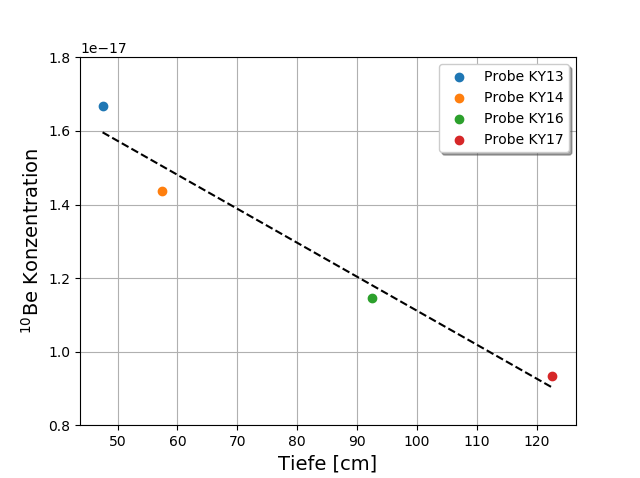
\includegraphics[width=0.7\linewidth]{Pictures/10be_konzentration.png}
  \caption{Berechnete Konzentration von $^9$Be in den Proben in Abhängigkeit von der Tiefe innerhalb der Probe, mit linearen Fit.}
  \label{deep}
\end{figure}
\clearpage
